\section{Jaudas detektora izstrāde}
Ir divas jaudas mērīšanas integrālās shēmas, kas veic atstarotās un izstarotās jaudas mērīšanu. R8 rezistors tiek izmantots, lai salāgotu ievades pretestību. C12 un C11 veido augstfrekvenču filtru un tam jābūt tādam, lai netiktu nogriezta 7.2 GHz frekvence. C10 keramiskais kondensators paredzēts vidējošanas funkcijas iekšējai RMS aprēķināšanai. Lai kompensētu temperatūras dreifēšanu, tiek izmantoti R6 un R7 rezistori pēc datu lapas ieteikumiem Rf signālam virs 5.8 GHz. R9 un R10 rezistori veido sprieguma dalītāju, lai panāktu 0.8 V uz VTGT, kas veido kompromisu starp precizitāti un maksimālu dinamisko diapozonu. C8, C9, C13 un C14 ir barošanas filtri. J8 ir SMA konektors, lai pieslēgtu mērāmo signālu.
\begin{figure}[H]
	\centering
    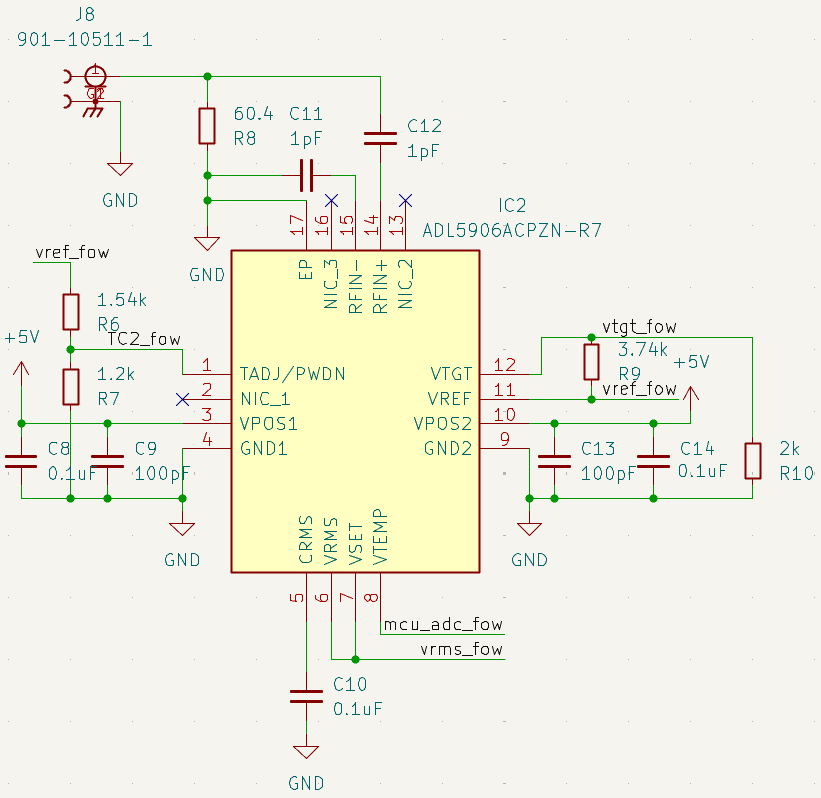
\includegraphics[width=0.5\textwidth]{pictures/fwd_powerdetector.png}\hspace{1cm}
    \caption{Jaudas noteikšanas integrālā shēma}
\end{figure}
Tika izveidota četru slāņu plate. Iespiedplates izstrādē liels uzsvars tika veikts uz pāris komponenšu izvēli, kondensatoru rezonanses frekvencei bija jābūt augstākai par mērāmo, celiņa platumam ieejā bija jābūt tādam, lai trakts būtu salāgots ar 50 ohm pretestību, SMA konektora kontaktlaukuma izmērs nedrīkstēja pārsniegt celiņa platumu, lai neveidotos signāla atstarojumi savienojuma vietā. Komponentes tika novietotas pēc iespējas tuvāk integrālajai shēmai, lai atbrīvotos no liekas parazītiskās induktivitātes. Trasējums veikts pēc datu lapas ieteikuma. 
\begin{figure}[H]
	\centering
    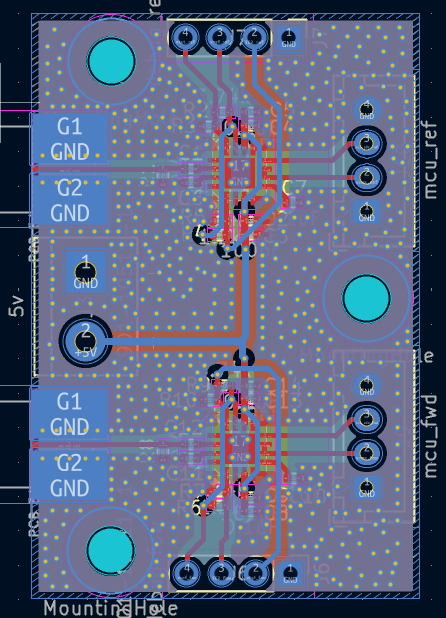
\includegraphics[width=0.6\textwidth]{pictures/board_powerdetector.png}\hspace{1cm}
    \caption{Jaudas noteikšanas iespiedplate}
\end{figure}
